\section{Slides de Aulas}

Nesta seção tratamos exclusivamente de slides destinados a apresentação de aulas completas sobre um assunto específico. Esse tipo de sequência é comum para professores.

\subsection{Que slides ter}

Os seguintes slides são recomendados para uma boa aula:
\begin{outline}
    \1 \textbf{Título da aula}, como na Figura \ref{fig:titulo};
    \1 \textbf{Objetivo da aula};
    \1 \textbf{Revisão} do que é necessário para entender a aula;
    \2 \textbf{Contextualizando} a aula curso
    \1 \textbf{Habilidades} específicas que serão aprendidas;
    \1 \textbf{Agenda} (ou Sumário);
    \2 A agenda ou sumário divide a aula em seções;
    \1 Um slide de \textbf{título para cada seção};
    \2 Pode ser o slide da agenda colocando ênfase na seção atual, como na Figura \ref{fig:meio};
    \1 Slides de conteúdo;
    \2 Não esqueça de uma motivação quando necessário;
    \2 Não esqueça do contexto histórico do que está sendo ensinado;
    \2 Não esqueça de definições
    \1 Pelo menos um slide com um exercício
    \2 Passar uma atividade de aprendizagem pós aula também é interessante, mesmo que ela nunca seja feita;
    \1 Slide de resumo, \textbf{``o que vimos hoje''}
    \2 Esse slide, ou slides, devem fechar a aula. Se necessário, por estar sobrando tempo, indique que agora, para reforçar, serão feitos ou discutidos exercícios, e siga por esse caminho até o fim do tempo;
    \1 \textbf{Referências} bibliográficas;
    \1 \textit{Preview} da \textbf{próxima aula}
\end{outline}



\begin{figure}[ht]
    \centering
    
\includegraphics[width=\tam\linewidth,frame]{imagens/capa.png}
    \caption{Um slide de título.}
    \label{fig:titulo}
\end{figure}

Outra boa sugestão é ter um slide, no início, que leve a pensar sobre o conteúdo da aula. Esse slide pode mostrar um problema real onde a técnica poderia ser aplicada, sendo algo do tipo ``como vocês fariam para fazer x?''. Isso seria adequado para uma aula onde se ensina o método PERT/CPM para calcular prazos de um projeto. Já em uma aula de programação inicial, que vai usar exemplos numéricos, poderia ser proposto um problema numérico, como achar números primos.

Ao mostrar um problema é interessante mostrar como ele pode se complicar. Ao mostrar um método de fazer algo que suplantou outro anterior, é interessante mostrar os problemas que o anterior tinha. Deve haver cuidado, porém, na estimativa de tempo, o contexto histórico deve ser limitado a motivação. Se começar do início de tudo, você acabará tendo menos tempo para falar do assunto que deve abordar e poderá perder pontos.

Eu agora também crio mais um slide, que fala sobre a metodologia da aula, e o tamanho da aula em slides e em tempo, como na Figura \ref{fig:metodologia}. Esse slide também mostra como símbolos podem ser usados para passar mensagens. Julgo ser  uma boa ideia mostrar isso também, inclusive porque não é uma prática comum entre os professores e pode surpreender positivamente.

\begin{figure}[htb]
    \centering
    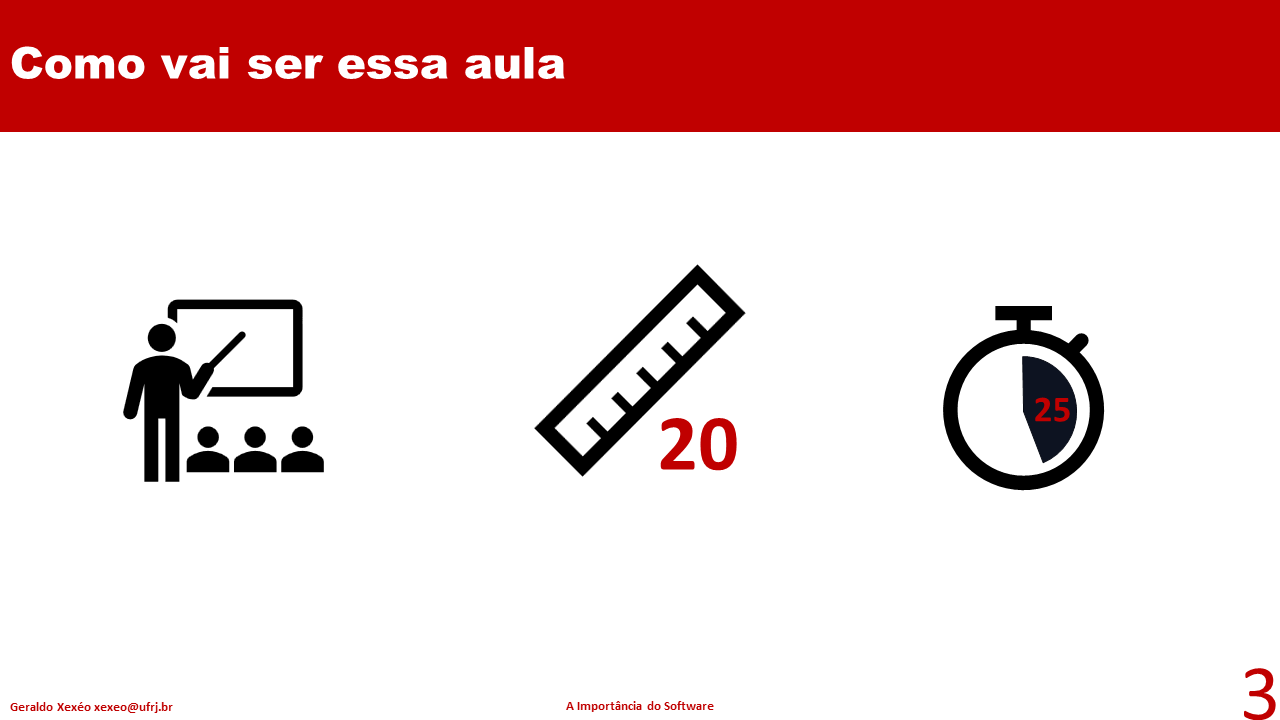
\includegraphics[width=\tam\linewidth,frame]{imagens/metodologia.png}
    \caption{Slide informando o aluno como vai ser a aula.}
    \label{fig:metodologia}
\end{figure}




\subsection{Estilo dos slides de aula}

A melhor estratégia para o estilo dos slides de aula \textbf{são o fundo branco, letras escuras, e cores para ressaltar}. Isso se adequa bem tanto a salas bem iluminadas quanto a salas escuras, para todo tipo de projetor. A Figura \ref{fig:teximag}, apesar de usar o forte grená, me parece bastante adequada. As outras figuras  mostram outros modelos que eu uso e sinto adequados para uma aula. As cores azuis e cinzas, porém, são mais ``fracas'' e podem levar a um pouco de monotonia.

Fundos devem ser evitados. Ele podem não aparecer como desejamos, causar efeitos que só aparecem na frequência do projetor, ou se confundir com linhas e letras do conteúdo.

\begin{figure}[hbt]
    \centering
    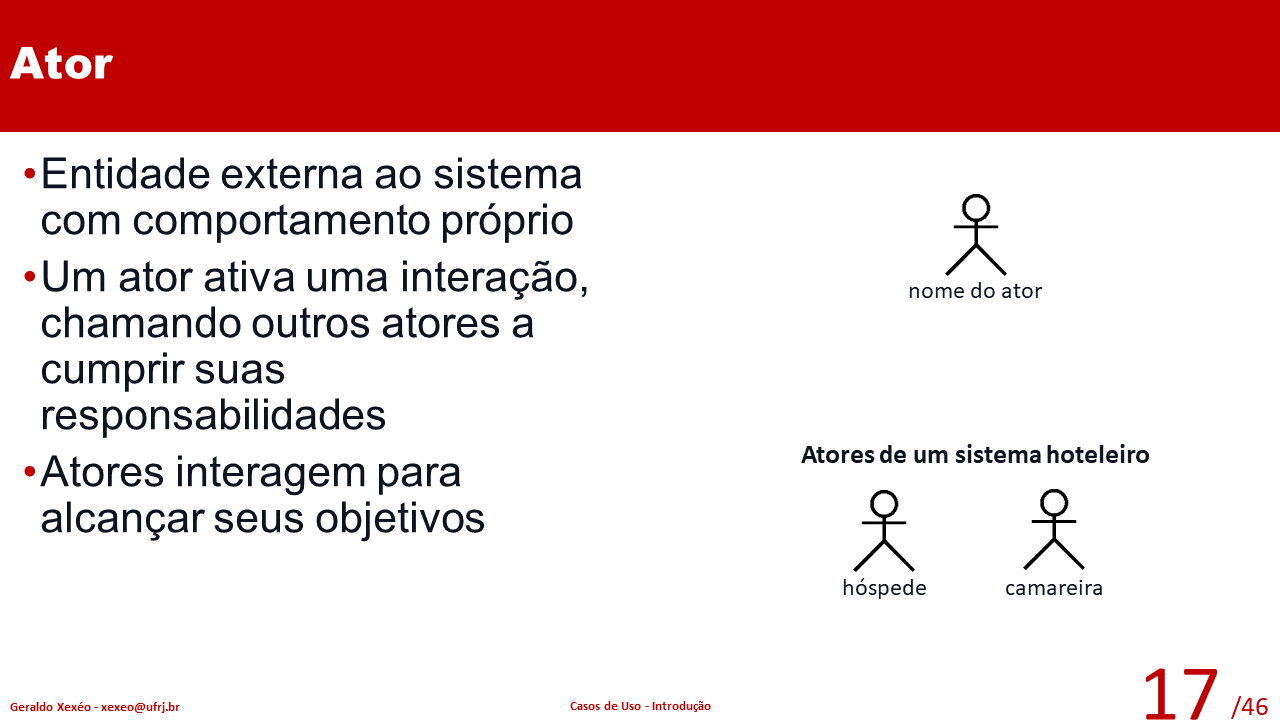
\includegraphics[width=\tam\linewidth,frame]{imagens/slidecomimage.png}
    \caption{Slide com texto e imagem}
    \label{fig:teximag}
\end{figure}

\subsection{Conteúdo dos slides}

Um slide para a aula tem como funções, em ordem decrescente de prioridade:
\begin{enumerate}
    \item servir de referência para o aluno e o professor no momento da aula;
    \item servir de guia para o estudo posterior, e
    \item servir de referência para os tópicos tratados, focando no conteúdo mais importante para a aula.
\end{enumerate}

O conteúdo típico de um slide é um lista de itens que indica o que o professor vai falar naquele momento. Essa lista pode conter exemplos, definições, motivação, dependendo da necessidade do slide.

Outro slide típico contém informações numéricas, na forma de gráficos e tabelas.

Forneça todas as referências, e \textbf{indique a propriedade intelectual de tudo}. Prefira imagens de domínio público ou com licenças amplas, como \textit{Creative Commons}.


